\documentclass{sigchi}

% Use this section to set the ACM copyright statement (e.g. for
% preprints). Consult the conference website for the camera-ready
% copyright statement.

% Copyright
\CopyrightYear{2020}
%\setcopyright{acmcopyright}
\setcopyright{acmlicensed}
%\setcopyright{rightsretained}
%\setcopyright{usgov}
%\setcopyright{usgovmixed}
%\setcopyright{cagov}
%\setcopyright{cagovmixed}
% DOI
\doi{https://doi.org/10.1145/3313831.XXXXXXX}
% ISBN
\isbn{978-1-4503-6708-0/20/04}
%Conference
\conferenceinfo{CHI'20,}{April 25--30, 2020, Honolulu, HI, USA}
%Price
\acmPrice{\$15.00}

% Use this command to override the default ACM copyright statement
% (e.g. for preprints). Consult the conference website for the
% camera-ready copyright statement.

%% HOW TO OVERRIDE THE DEFAULT COPYRIGHT STRIP --
%% Please note you need to make sure the copy for your specific
%% license is used here!
% \toappear{
% Permission to make digital or hard copies of all or part of this work
% for personal or classroom use is granted without fee provided that
% copies are not made or distributed for profit or commercial advantage
% and that copies bear this notice and the full citation on the first
% page. Copyrights for components of this work owned by others than ACM
% must be honored. Abstracting with credit is permitted. To copy
% otherwise, or republish, to post on servers or to redistribute to
% lists, requires prior specific permission and/or a fee. Request
% permissions from \href{mailto:Permissions@acm.org}{Permissions@acm.org}. \\
% \emph{CHI '16}, May 07--12, 2016, San Jose, CA, USA \\
% ACM xxx-x-xxxx-xxxx-x/xx/xx\ldots \$15.00 \\
% DOI: \url{http://dx.doi.org/xx.xxxx/xxxxxxx.xxxxxxx}
% }

% Arabic page numbers for submission. Remove this line to eliminate
% page numbers for the camera ready copy
% \pagenumbering{arabic}

% Load basic packages
\usepackage{balance}    % to better equalize the last page
\usepackage{graphics}   % for EPS, load graphicx instead 
\usepackage[T1]{fontenc}  % for umlauts and other diaeresis
\usepackage{txfonts}
\usepackage{mathptmx}
\usepackage[pdflang={en-US},pdftex,breaklinks]{hyperref}
\usepackage{color}
\usepackage{booktabs}
\usepackage{textcomp}
\usepackage{url}
\def\UrlBreaks{\do\/\do-}
\usepackage{breakurl}
\usepackage{multirow}
\usepackage{dblfloatfix}
\usepackage[super]{nth}

% Some optional stuff you might like/need.
\usepackage{microtype}    % Improved Tracking and Kerning
% \usepackage[all]{hypcap}  % Fixes bug in hyperref caption linking
\usepackage{ccicons}     % Cite your images correctly!
% \usepackage[utf8]{inputenc} % for a UTF8 editor only

% If you want to use todo notes, marginpars etc. during creation of
% your draft document, you have to enable the "chi_draft" option for
% the document class. To do this, change the very first line to:
% "\documentclass[chi_draft]{sigchi}". You can then place todo notes
% by using the "\todo{...}" command. Make sure to disable the draft
% option again before submitting your final document.
\usepackage{todonotes}

% Paper metadata (use plain text, for PDF inclusion and later
% re-using, if desired). Use \emtpyauthor when submitting for review
% so you remain anonymous.
\def\plaintitle{Exploring the Potential of Open Data Portals to Address the Information Needs of Lay Citizens}
\def\plainauthor{First Author, Second Author, Third Author,
 Fourth Author, Fifth Author, Sixth Author}
\def\emptyauthor{}
\def\plainkeywords{Open data, information seeking, user study}

% llt: Define a global style for URLs, rather that the default one
\makeatletter
\def\url@leostyle{%
 \@ifundefined{selectfont}{
  \def\UrlFont{\sf}
 }{
  \def\UrlFont{\small\bf\ttfamily}
 }}
\makeatother
\urlstyle{leo}

% To make various LaTeX processors do the right thing with page size.
\def\pprw{8.5in}
\def\pprh{11in}
\special{papersize=\pprw,\pprh}
\setlength{\paperwidth}{\pprw}
\setlength{\paperheight}{\pprh}
\setlength{\pdfpagewidth}{\pprw}
\setlength{\pdfpageheight}{\pprh}

% Make sure hyperref comes last of your loaded packages, to give it a
% fighting chance of not being over-written, since its job is to
% redefine many LaTeX commands.
\definecolor{linkColor}{RGB}{6,125,233}
\hypersetup{%
 pdftitle={\plaintitle},
% Use \plainauthor for final version.
% pdfauthor={\plainauthor},
 pdfauthor={\emptyauthor},
 pdfkeywords={\plainkeywords},
 pdfdisplaydoctitle=true, % For Accessibility
 bookmarksnumbered,
 pdfstartview={FitH},
 colorlinks,
 citecolor=black,
 filecolor=black,
 linkcolor=black,
 urlcolor=linkColor,
 breaklinks=true,
 hypertexnames=false
}

% create a shortcut to typeset table headings
% \newcommand\tabhead[1]{\small\textbf{#1}}

% End of preamble. Here it comes the document.
\begin{document}

\title{\plaintitle}

\numberofauthors{7}
\author{%
 \alignauthor{Leave Authors Anonymous\\
  \affaddr{for Submission}\\
  \affaddr{City, Country}\\
  \email{e-mail address}}\\
 \alignauthor{Leave Authors Anonymous\\
  \affaddr{for Submission}\\
  \affaddr{City, Country}\\
  \email{e-mail address}}\\
 \alignauthor{Leave Authors Anonymous\\
  \affaddr{for Submission}\\
  \affaddr{City, Country}\\
  \email{e-mail address}}\\
 \alignauthor{Leave Authors Anonymous\\
  \affaddr{for Submission}\\
  \affaddr{City, Country}\\
  \email{e-mail address}}\\
 \alignauthor{Leave Authors Anonymous\\
  \affaddr{for Submission}\\
  \affaddr{City, Country}\\
  \email{e-mail address}}\\
 \alignauthor{Leave Authors Anonymous\\
  \affaddr{for Submission}\\
  \affaddr{City, Country}\\
  \email{e-mail address}}\\
 \alignauthor{Leave Authors Anonymous\\
  \affaddr{for Submission}\\
  \affaddr{City, Country}\\
  \email{e-mail address}}\\
}

\maketitle

\begin{abstract}
Open government data allows for transparency from governments and access to data collected about its citizens. However, we are still far from achieving universal citizen participation because data literacy and experience are necessary to extract insights from data. There is also no guarantee if available data can address people's information needs. We explored the potential of open government data portals in addressing the information needs of citizens through an online survey and found that these can only be partially answered by the available data. To understand their information seeking behavior, we conducted usability tests of open data portals with 21 citizens, and used semi-structured interviews to identify gaps in the portals' design. We found that citizens would benefit from: localized and advanced search engines; and visualized, contextualized, and processed content for better sensemaking. We conclude with design guidelines for open data portals catered to citizens.
\end{abstract}


% ACM Classfication

\begin{CCSXML}
<ccs2012>
<concept>
<concept_id>10003120.10003121</concept_id>
<concept_desc>Human-centered computing~Human computer interaction (HCI)</concept_desc>
<concept_significance>500</concept_significance>
</concept>
<concept>
<concept_id>10003120.10003121.10003122.10003334</concept_id>
<concept_desc>Human-centered computing~User studies</concept_desc>
<concept_significance>300</concept_significance>
</concept>
<concept>
<concept_id>10003120.10003121.10003122.10010854</concept_id>
<concept_desc>Human-centered computing~Usability testing</concept_desc>
<concept_significance>100</concept_significance>
</concept>
</ccs2012>
\end{CCSXML}

\ccsdesc[500]{Human-centered computing~Human computer interaction (HCI)}
\ccsdesc[300]{Human-centered computing~User studies}
\ccsdesc[100]{Human-centered computing~Usability testing}

% Author Keywords
\keywords{\plainkeywords}

% Print the classficiation codes
\printccsdesc
% Please use the 2012 Classifiers and see this link to embed them in the text: \url{https://dl.acm.org/ccs/ccs_flat.cfm}

\section{Introduction}
% What is open data? Last sentence can state that governments are the biggest implementers of this movement.
By definition, \textit{open data} should be machine-readable, free to use, share, modify, and analyze by anyone \cite{corrales2019knowledge, DAWES201615}. Publishing open data was first started by Robert King Merton when he pushed for the open sharing of scientific data \cite{chignard2013}. On the other hand, the term "\textit{open government}" was first used in the fifties and was generally used to refer to making previously confidential government information public with the goal of making governments more politically transparent \cite{YuRobinson2012}. 

% How are governments opening up their data? Highlight the 2 practices being implemented: Open Data and FOI
Through the advancement of the Internet and web technologies combined with the growing clamor of citizens and technologists to engage and innovate, governments started to adapt technology to make data more accessible through open government data (OGD) portals \cite{DAWES201615, YuRobinson2012}. In contrast, lobbyists of Freedom of Information (FOI) seek for governments to establish constitutional guarantees for a "right-to-know" process. In the absence of publicly available government data, a passed FOI law ensures data requesters that they will get a response within a specified number of days. However, it is still the discretion of the government agencies whether or not they will provide the data. 

% How are open data being utilized? Sample applications like Sakay.ph, etc. Emphasize that these are mainly intermediaries that use data for businesses, research and development work. 
In countries with rich open data, we can see these being actively used for policy, research, and civic innovations. Projects like Citygram\footnote{\url{https://www.citygram.org/}} in the USA allows citizens to get updated with recent reports in their area while GoodGuide\footnote{\url{https://www.goodguide.com}} in the EU lets users check how healthy grocery items are. Several technology companies, such as Sakay.ph\footnote{\url{https://sakay.ph/}} and Rentlogic\footnote{\url{https://www.rentlogic.com/}}, maximized OGD in developing solutions that provide commute routes in the Philippines and apartment building ratings in New York, respectively. Even in other developing countries, various case studies have been conducted to showcase the potential of open data \cite{farahi2018}. Although the impact was not quantified, further research is encouraged to evaluate the effects of OGD in developing countries \cite{farahi2018}. However, despite the growing trend of open data use, these projects were mostly developed by third-party intermediaries that use data for business, research, and development. 

% What do current reports on open data reveal? Who is it supposed to provide data for? That we still lack in achieving universal participation, etc.
% What do governments focus in designing these portals? We can end the paragraph with "With the current focus of how these portals are designed and implemented, HCI research has the potential to address these gaps by answering the following questions:"
Open data is perceived to be a useful tool for citizens, in general, to demand a more open and collaborative government \cite{warwick2017}. Despite the presence of guidelines for transparency and citizen engagement from the United Nations \cite{UN2013}, a gap still exists in utilizing OGD for citizen engagement. It has been argued that most OGD users have the technical capabilities to analyze data in its raw formats \cite{DAWES201615}. This may be attributed to the fact that open data should be machine-readable which requires some technical understanding of computer processing. With the current focus of how these portals are designed and implemented, human-computer interaction (HCI) research has the potential to address these gaps by answering the following questions:
\begin{itemize}
  \item RQ1: Does existing open government data support the information needs of citizens? Why or why not?
  \item RQ2: Is the existing information seeking behavior of citizens applicable to open data portals? Why or why not?
  \item RQ3: How effective are open government data portals in supporting the information seeking and sensemaking needs of the citizens?
\end{itemize}

To answer the first research question, we conducted a survey to explore the information needs of Filipino citizens and evaluated if these needs could be answered by existing OGD. To answer the other two research questions, a usability experiment on Philippine open data portals followed by semi-structured interviews helped to identify gaps in the portals' design. We recruited 21 participants based on convenience but priority was given to lay citizens with little to no experience with data analysis.

% we conducted semi-structured interviews with 21 individuals to observe their information seeking and sensemaking behavior through predetermined tasks. 

% proposed revised version of commented section tagged by kyle
We first discuss the information needs of lay citizens and how OGD might contribute to these needs. We found that OGD can support some of the information needs of lay citizens, but these data would require organization and processing to be presented as information. We then examine the information seeking behavior of lay citizens and data workers to determine whether OGD portals support the said behavior. We observed that lay citizens primarily rely on localized and advanced search engines to retrieve answers to their concerns. Additionally, our results suggest that citizens benefit from visualized, contextualized, and processed content regardless of the experience with data work. This study builds on existing research to understand how to better design OGD portals for its users \cite{Choi2017, Erete2016, kacprzak2019characterising, Koesten2019, Koesten2017}, specifically how to cater to lay citizens to promote universal citizen participation for open government.

% We found that OGD can support some of the information needs of lay citizens, but these data would require organization and processing to be presented as information. We also observed that lay citizens value localized and advanced search engines to find the answers to their concerns. Our results also suggest that regardless of the experience with data work, citizens benefit from visualized, contextualized, and processed content. We first discuss the information needs of lay citizens and how OGD might contribute to these needs. We then look into the information seeking behavior of lay citizens and data workers to identify gaps in current OGD portals to support sensemaking. This study serves as our formative research in understanding how to improve the presentation of OGD for lay citizens to promote citizen engagement.

\section{Related Work}
A survey of research in OGD implementation and human-data interaction (HDI) suggests the need for insights from lay citizens since they are also the target users of OGD portals \cite{warwick2017}. While existing HCI research provides ways of improving OGD portals for experienced data users, understanding the behavior of lay citizens in contrast with data users presents an opportunity to better design inclusive OGD portals and other supplementary tools. 

\subsection{OGD Portal Evaluation}
% to support yung statement natin sa taas na ito lang finofocus ng mga governments when they try to measure success of their portals
Most research conducted around OGD portals focused on the implementations of developed countries \cite{kacprzak2019characterising, klimek2019dcat, Koesten2019,Parycek2014}. Using the Global Open Data Index (GODI) as a reference, countries evaluated in these studies are within the top 30 out of 94 countries \cite{godimetric2016}. This index only measures the openness of data published according to guidelines under \textit{Open Definition} \cite{godimetric2016}.

Evaluating the quality of data provided is important for data projects. It was shown that having a standardized format in publishing metadata of open data is valuable in promoting usability, portability, availability, and performance as well as supplementing work on Linked Open Data \cite{klimek2019dcat}. In addition to the published data, understanding the feedback from the targeted users is also critical to evaluate implementations of OGD portals. Parycek et al. \cite{Parycek2014} evaluated Vienna's OGD implementation through understanding the perspectives from both internal and external stakeholders in terms of the process, requirements, and benefits. By understanding these perspectives, policy makers would know how to improve their current implementation. Our study further contributes to this field by focusing on the needs and understanding of citizens.

\subsection{HCI for Open Data}
User studies of OGD portals are currently focused on data workers or individuals who are experts in processing these kinds of data \cite{Choi2017, Erete2016, kacprzak2019characterising, Koesten2019, Koesten2017}. They are usually from open data intermediaries, like civic start-ups and infomediaries, that usually take the role of aggregators, developers, enrichers, and enablers \cite{VanSchalkwyk2015}. Despite these early works, current OGD portals are still lacking in terms of advanced search systems \cite{kacprzak2019characterising, Koesten2017} and consideration for collaborative work \cite{Choi2017, Erete2016, Koesten2019}.

\subsubsection{Data Search}
Koesten et al. \cite{Koesten2017} suggested a framework on how data workers interact with data to show that behaviors are dependent on the requirements of the task. Different tasks would require specific search strategies such as web search, data portal search, FOI data request, and consulting other data workers. Despite the existence of data portals, majority of the participants reported using Google to find the data they needed. While this may not seem too surprising with our over-dependence on big search engines, it does suggest how lacking as a central resource these portals are designed and implemented. To understand further the information seeking behavior of the users, a follow up study analyzed dataset search queries together with crowd sourced queries \cite{kacprzak2019characterising}. Our study reiterates the need to redesign data search environments to be more suggestive and include spatial and temporal filtering.

\subsubsection{Designs for Collaborative Work}
Collaborative work using OGD is interdisciplinary by nature \cite{Choi2017}. Proper data documentation, conversation, change control, and custom data access were identified as user needs for effective collaboration with structured data \cite{Koesten2019}. While these studies provide great insight to how open data portals may be improved for better collaboration between data workers, little research has explored the potential for lay citizens. When open data use in non-profit organizations were evaluated, people with less contact with data tend to rely on expert data analysts to be able to understand the data provided \cite{Erete2016}. From these findings, we see an opportunity for HCI to analyze how open data portals may be improved for individuals with limited exposure to data.

\section{Philippine Open Government Data}
Building on a previous study, which showed that people better identify with data when associated with a location \cite{Puussaar2018}, we chose Open Data Philippines\footnote{\url{https://data.gov.ph/}} (ODPH) and the Freedom of Information\footnote{\url{https://foi.gov.ph}} (eFOI) website of the Philippines to assess the efficacy of OGD portals in supporting the information needs of citizens. 

\subsection{Open Data Philippines}
% parang quick description ng kung nasan na yung implementation nung portals, ano yung current na laman, etc.
The official open data portal of the Philippines was launched in January 2014 in fulfilment to the commitments of the country to provide open data to its citizens \cite{ODPH2015}. The portal is running under DKAN which is a Drupal-based implementation of CKAN (Comprehensive Knowledge Archive Network) \cite{dkan2019}. The platform hosts data provided by different agencies and allows users to search, preview, and download these without any restrictions. Users may also browse the catalog by category or by agency. In the dataset preview, users may also create exploratory graphs with the fields available in the file.

% Despite the extensive usage of civil society organizations and the private sector, OGD in the Philippines still suffers from low utilization which suggests a disconnect between the published data and the information needs of the citizens \cite{galindesZaplan2018}. 

\subsection{Electronic Freedom of Information}
In 2016, an executive order from the President of the Philippines, Rodrigo Duterte, made the executive branch of the government comply with the people's rights to information \cite{duterte2016}. With this, the Electronic Freedom of Information portal was launched on November 2016 \cite{cigaral2016}. This portal serves as an electronic tracker of citizen requests for information about government transactions and operations. eFOI requires citizens to provide a valid email address and any valid government identification as proof of identity prior to making a request. Requests must be directed to the correct agency otherwise it would be rejected. After a request has been filed, an email would be sent notifying the requester of the status. Citizens may also browse through existing requests. Each request shows a conversational thread of the FOI officer and the corresponding agency. 

\section{Climate Survey and Portal Analysis}
We conducted a 15 to 20 minute climate survey to gauge the awareness and the interest of Filipinos about the open government initiatives of the country, specifically ODPH and eFOI. We also conducted an inventory analysis of the available data in ODPH. The survey was released in July 2019 and closed in August 2019 through Google Forms. Participant consent was acquired prior to proceeding with the questionnaire as per institutional ethical research requirements.

\begin{table}[t]
  \centering
  \begin{tabular}{l p{5.85cm}}
     \toprule
     \textbf{\textit{Level}} & \textbf{\textit{Scenario}} \\
     \midrule
     Personal & Suppose you want to live in a new apartment in Makati City, and you want to know how safe the area is before making a decision.\\
     \midrule
     Extrapersonal & Suppose you or your child wants to study in a state university within Metro Manila. Before making a decision, you want to know which state university has an acceptable faculty/student ratio.\\
     \midrule
     Impersonal & Suppose you want to know where most Philippine presidents go for their foreign trips.\\
     \bottomrule
  \end{tabular}
  \caption{Information seeking scenarios}
  \label{tab:scenarios}
\end{table}

\subsection{Survey Design}
We designed our survey to be as extensive as possible in understanding the factors that could potentially drive the awareness of Filipinos about open government initiatives. Prior to asking about their awareness of ODPH and eFOI, we asked them if they had experience with data analysis to determine if there is a relationship between experience and awareness of open data portals. 

% For data analysis experience, we asked our participants where they had used data before. Choices provided were for their main occupation, as a paid part-time job, as a hobby, as a passion or advocacy, for curiosity, and a final option of any other type of work. 
% Based on a previous study, most data analysis work done are descriptive and exploratory and less inferential and predictive\cite{Choi2017}. Using this information, we also asked how often they performed descriptive, diagnostic, prescriptive, and predictive analyses with their data for each type of data work they did.

To understand the information seeking behavior of Filipinos, we provided three scenarios with different degrees of personal involvement in decision making. Table \ref{tab:scenarios} lists the specific scenarios we provided in the survey. The personal scenario involves making a decision involving oneself. The extrapersonal scenarios may affect the individual to some extent but is more focused on another person. Lastly, the impersonal scenario involves looking for information that is more detached from their personal lives. We asked them which information sources they would most likely consult in making these decisions.

Finally, we provided a brief description of ODPH and eFOI prior to asking if they have ever heard of or used these two portals. We used a 5-point Likert scale to measure the frequency and usefulness of the portals for those who have at least visited or used them. In the end, we asked them to provide three sectors of government they would be most interested in to help us determine whether the interests of the citizens align with what is provided by the government.

\subsection{Participants}
The only requirement to participate in our survey was to be a Filipino citizen. We utilized snowball sampling by distributing the survey through Facebook, Twitter, and different Facebook Groups to further our reach. We also made a Filipino version of the survey to cater to the non-English speaking citizens of the country. We were able to collect a total of 119 valid response both forms with six of them coming from the Filipino survey.

More than half (N=63) of our respondents were women. The average age was 33 (SD=13.77). Majority of the respondents were students (N=30), professionals in Information Techno logy (N=22), and professionals in Business Consulting and Management (N=15). We also got respondents from different sectors as to gain varied insights. As a result, more than half (N=69) responded to having done data work as part of their main occupation in the past 12 months. Some respondents (N=54) even reported doing data work in more than one of the categories provided.

\subsection{Survey and Data Portals Analysis}
% Paolo is writing here.
To see if existing government data portals support the information needs of the citizens (RQ1), we must also understand the open data available. We created an inventory of the 273 datasets in ODPH and individually investigated the files. We manually identified the spatial and temporal granularity, if available, of the datasets as a measure of how detailed they were.

In addition to the categories provided, we also asked our respondents what other relevant questions they might have for the next 12 months. Since this was a free-form text field, we manually classified 96 responses according to the themes that emerged. After categorizing each response, we individually assessed if they can be answered by available data from ODPH and eFOI. We also considered whether or not the data for the questions may be found on other government portals or may be requested in eFOI.

% Kyle will write the results of the survey
\subsection{Results}
We start by discussing the unanticipated issues encountered during the analysis of our climate survey and available open data. To address whether or not OGD portals serve the needs of lay citizens, we provide an understanding of the information needs of our respondents. We then use the results from the survey and the data inventory to answer why or why not these needs are being met (RQ1).

\subsubsection{Issues Encountered}
% We raise some unanticipated issues that could arise from a climate survey that targets any Filipino citizen. Through no control over the responses that will be provided by the citizens, several erroneous or ambiguous answers to the questions were given. These answers were taken and grouped during analysis to prevent any unneeded assumptions. However, our study prevents these ambiguities from affecting the overall result of the climate survey.

We had open-ended questions in our survey which inquired about the respondent's personal interests. As a result, several erroneous or ambiguous answers to the open-ended questions were given. To prevent further ambiguities, we grouped these answers during analysis to prevent any unneeded assumptions.

Additionally, we also had conflicting responses with the data experience and the level of awareness. We found two individuals who said they were fully aware and have used the open data portals but did not have any data analysis work done in the past 12 months. Although all our questions were framed with the same time period, we acknowledge there could have been issues with the phrasing that caused this conflict.

Another issue encountered was the unexpected redesign of ODPH. Datasets were initially under nine different categories which we used in our climate survey. However, the portal was redesigned sometime in late August 2019 after we collected the responses for our study. We were still in the process of finalizing our data inventory when the redesign occurred; therefore, the datasets were categorized according to the 20 new categories in the updated portal. We acknowledge the conflict in semantics between categories, however, these differences are minimal.

% To answer our first research question, we must first understand the information needs and level of awareness of the citizens. We defined the information needs as the interests of the citizen based on a list of categories taken from Open Data Philippines categories and awareness into 4 categories: (1) Fully aware and used the portal, (2) Aware and have visited the portal, (3) Has heard about the portal, and (4) Did not know about the portal.
\subsubsection{Gauging Awareness of Open Data Portals}
To gauge the level of awareness of the ODPH and eFOI, we classified awareness into four categories: (1) fully aware and used the portal, (2) aware and have visited the portal, (3) has only heard about the portal, and (4) did not know about the portal completely. We found that people were generally more aware of ODPH than eFOI. However, after a pairwise comparison, we found that majority of citizens (N=39) were unaware while only a few (N=11) were aware of both portals. In terms of educational attainment, respondents who have used the datasets from ODPH had either a Bachelor's degree (N=5) or higher (N=7). However, of the 13 respondents who have used eFOI, two respondents have already requested datasets from eFOI even though they have no Bachelor's degree. 

We conducted $\chi^2$ tests of independence on (1) the levels of awareness between the two portals and (2) between the experience in data work and the level of awareness of each portal. We found that awareness of one data portal is dependent on the awareness of the other data portal and that awareness is independent from having experience with data work.

% We conducted a $\chi^2$ test of independence between the level of awareness of the two portals and found that awareness of one data portal is dependent on the awareness of the other data portal. We also conducted a $\chi^2$ test of independence between the level of awareness of each portal and their experience with data work. We found that awareness is independent from having experience with data work. 

\subsubsection{Understanding Citizen Information Needs}
To easily associate the information needs of citizens with available open data, we used the categories from ODPH. We found that most Filipino citizens are interested in Business and Economics (N=62), Transport (N=56), and Disaster and Rehabilitation/Environment (N=45). The profession of those who chose the three categories were mostly students and IT professionals. When comparing data work experience, we see that data workers are interested in Business and Economics while those with no data experience are interested in Security. In addition to the categories, we asked our respondents what relevant questions they would have in the next 12 months. There were varied responses but common themes that emerged were related to \textit{real estate}, specifically where to move, \textit{transportation}, \textit{economy}, \textit{disaster risks}, and \textit{employment}. 

We believe that these top categories represent some aspect of the personal lives of the citizens. Business and economics is closely associated with financial matters and is a basic commodity in life. Almost all of our respondents come from the Greater Manila area, which comprises of Metro Manila and contiguous urban areas such as Laguna, Cavite, Rizal, Pampanga, and Bulacan. The need to commute contributes to the interest in transportation especially with the growing traffic congestion problems of the area \cite{Traffic55:online, Expertsa90:online}. Interest in disaster rehabilitation and environment could be attributed to the fact that the Philippines is a disaster prone country due to prominent flooding and proximity to the Pacific Ring of Fire \cite{WhyPhili58:online}.

\subsubsection{Usefulness of Open Data Portals}
We used a 5-point Likert scale to determine the search frequency of those who have used the portal and the usefulness of the data to them. The overall response was that the data provided was \textit{"either incomplete or non-existent"}: 

\begin{quote}
  "Especially in the [Philippines], most available datasets are outdated or incomplete. Because of these issues, a lot of times, these are unsuitable to be used in the projects."
\end{quote}

Out of the 11 respondents that were aware of both portals, only one respondent, a government employee, preferred eFOI over ODPH. When asked for the rationale for his sentiment on ODPH, he stated that he \textit{"didn't have time and inclination"} to search. Although he's never requested data from eFOI personally, he said, \textit{"I love the [eFOI] interface"}. 

\subsubsection{Available Data}
Out of the 273 available datasets, most published data is related to the National Government (N=57). These datasets are mostly statistics from the National Statistical Coordination Board (NSCB), electoral results from the Commission on Elections, and government spending balances from the Department of Budget and Management. Education and Training, Banking and Finance, and Transportation are tied with 34 datasets each. 

Most of the datasets related to business and economics would be banking and finance data. However, the available datasets in ODPH are mostly annual bank level information. Transport data covers air, sea, and rail transport. Air transport includes cargo and passenger movement on a monthly granularity. The most noteworthy transport dataset available is hourly passenger traffic of the Metro Rail Transit (MRT) for certain years. As for environment and disaster rehabilitation related datasets, there are only five datasets available. From the five available datasets, three are expenditure reports from the Climate Change Commission while the other two are the number of policies approved annually by the Land Management Bureau and Philippine Forest Coverage statistics. 

% In line with the most common dataset based on the respondent's answers, we inspected if each data for Business and Economics, Transport, and Environment is complete. We found that there are 20 out of the 34 (58.8\%) completed data for Business and Economics, 22 out of 34 (64.7\%) completed data for Transportation, and 2 out of the 5 (40\%) completed data for Environment.

The ODPH categories provide only a high-level understanding of the interests of the respondents. However, given that most data are either national, regional, provincial, or specific to a single location, these datasets may not be useful for most people. The most common response to the open-ended question was deciding where to move (N=18). Transportation related responses (N=15) involved travel routes, improvement to public transportation, and alternative transportation development such as bike lanes. Economic related responses (N=10) revolved around inflation and the overall economic development of the country. Since responses had varying detail, we classified these as \textit{"answerable"} based on whether or not existing datasets can potentially answer their query. To illustrate, we considered crime statistics as a potential dataset to represent safety associated with moving into a new city. Based on our classification, we found that 24 out of 107 (22.43\%) responses may potentially be answered in part by available datasets in ODPH. 

By simply looking at the quantity and the granularity of the datasets available, we believe that there is potential for these OGD portals to support the information needs of certain citizens. However, further studies and analyses must be done to evaluate how effective these portals are in supporting their needs. 

\subsubsection{Information Sources}
To see where citizens commonly look for information based on the scenarios provided in Table \ref{tab:scenarios}, we used a 5-point Likert scale to ask them how likely they would consult (1) family and friends, (2) Google, (3) government websites, (4) news websites, (5) print news, (6) social media, and (7) university research websites. For the personal scenario, respondents preferred getting firsthand information from \textit{family and friends} over other sources. In the extrapersonal scenario, \textit{Google} and \textit{family and friends} were the most likely sources. In the impersonal scenario, respondents refer to \textit{news websites} and \textit{Google}. When asked if they had any other data-related inquires, \textit{Google} was the main information source for majority of the respondents (N=77; 64.71\%). From these results, people have a high dependency on big search engines. 

% \begin{table*}[t]
%  \centering
%  \begin{tabular}{l p{6.3cm} p{6.5cm}}
%   \toprule
%   \textbf{\textit{Portal}}
%   & \textbf{\textit{Personal Task}}
%   & \textbf{\textit{Impersonal Task}}\\
%   \midrule
%   Open Search & How prevalent is crime in the province where you live? & Find the number of students enrolled in the University of the Philippines during 2015.\\
%   \midrule
%   Open Data Philippines & How much, in Philippine Peso, was lost due to fire in your city of residence in 2013? & What are the top countries that most Philippine presidents go to as part of their work? \\
%   \midrule
%   Freedom of Information & How many people have work in your region? & How many road accidents happened in Metro Manila in 2018?\\
%   \bottomrule
%  \end{tabular}
%  \caption{List of search tasks performed by the participants per portal.}~\label{tab:searchtasks}
% \end{table*}

\section{Usability Experiment}
To further examine the information seeking behavior of lay citizens, we conducted usability experiments of ODPH and eFOI. These experiments were done in parallel with semi-structured interviews to identify gaps in the design of the portals. The interviews were conducted between July and August 2019 at locations convenient to the participants. Participant consent was obtained prior to conducting the interview. Dialogues were audio recorded while the on-screen behavior was recorded using a screen capture software. 

\subsection{Participants}
For this study, our participants were selected based on their availability to be interviewed during the study period. We focused on recruiting individuals with (1) less than a year of experience with data analysis and (2) no experience using OGD portals for any kind of work. For participants that meet either criteria, they were classified as a \textit{lay person}. Otherwise, we identified them as \textit{data workers}. As shown in Table \ref{tab:participants}, we were able to successfully recruit 13 lay people and eight data workers for our interviews, however, two of the lay people expressed their lack of experience in working with computers in general. Majority (N=14) of our participants were men. The average age for all participants was 31 (SD=15.08). We had nine student participants and five individuals working in local government.

% Please add the following required packages to your document preamble:
% \usepackage{graphicx}
\begin{table*}[t]
\centering
\resizebox{\textwidth}{!}{%
\begin{tabular}{llr|ccc|ccc|ccc}
\toprule
\textbf{} & \textbf{} & \multicolumn{1}{l|}{\textbf{}} & \multicolumn{3}{c|}{\textit{\textbf{Open Search}}} & \multicolumn{3}{c|}{\textit{\textbf{Open Data PH}}} & \multicolumn{3}{c}{\textit{\textbf{eFOI}}} \\
\textit{ID} & \textit{Occupation} & \multicolumn{1}{l|}{\textit{Age}} & \multicolumn{1}{l}{\textit{Completed}} & \multicolumn{1}{l}{\textit{\begin{tabular}[c]{@{}c@{}}Total Time\\ (mm:ss)\end{tabular}}} & \multicolumn{1}{l|}{\textit{\begin{tabular}[c]{@{}c@{}}Queries \\ per minute\end{tabular}}} & \multicolumn{1}{l}{\textit{Completed}} & \multicolumn{1}{l}{\textit{\begin{tabular}[c]{@{}c@{}}Total Time\\ (mm:ss)\end{tabular}}} & \multicolumn{1}{l|}{\textit{\begin{tabular}[c]{@{}c@{}}Queries \\ per minute\end{tabular}}} & \multicolumn{1}{l}{\textit{Completed}} & \multicolumn{1}{l}{\textit{\begin{tabular}[c]{@{}c@{}}Total Time\\ (mm:ss)\end{tabular}}} & \multicolumn{1}{l}{\textit{\begin{tabular}[c]{@{}c@{}}Queries \\ per minute\end{tabular}}} \\ \midrule
DW1 & Revenue Assurance Manager & 34 & 2 & 07:08 & 1.12 & 2 & 03:35 & 1.40 & 2 & 09:07 & 0.88 \\
DW2 & Professor & 30 & 2 & 03:20 & 1.20 & 0 & 03:31 & 2.84 & 2 & 07:02 & 1.00 \\
DW3 & Student & 23 & 2 & 06:33 & 0.92 & 2 & 06:13 & 0.48 & 2 & 04:59 & 0.80 \\
DW4 & Senior Data Engineer & 34 & 1 & 04:23 & 1.14 & 2 & 02:09 & 0.93 & 1 & 04:01 & 0.50 \\
DW5 & Student & 19 & 1 & 06:20 & 0.95 & 1 & 03:19 & 1.21 & 1 & 08:33 & 0.82 \\
DW6 & Student & 19 & 2 & 03:13 & 0.93 & 2 & 03:02 & 1.32 & 2 & 06:41 & 1.05 \\
DW7 & IT Consultant & 62 & 2 & 04:23 & 0.68 & 2 & 08:16 & 0.48 & 0 & 01:58* & 1.53 \\
DW8 & Baranggay Kagawad & 29 & 2 & 07:10 & 0.56 & 2 & 08:30 & 0.71 & 2 & 14:29 & 0.21 \\
 & \textbf{Average}  & \textbf{31.25}  & \textbf{87.50\%}  & \textbf{05:19} & \textbf{0.94}  & \textbf{81.25\%}  & \textbf{04:49} & \textbf{1.17}  & \textbf{75.00\%}  & \textbf{07:50} & \textbf{0.75}  \\ 
\midrule
L1 & Student & 20 & 2 & 13:45 & 0.80 & 2 & 05:21 & 0.93 & 1 & 05:00 & 1.20 \\
L2 & SK Chairman & 23 & 2 & 07:21 & 0.41 & 2 & 11:13 & 0.09 & 0 & 16:44 & 0.48 \\
L3 & Student & 20 & 1 & 09:07 & 0.55 & 2 & 08:56 & 1.12 & 1 & 13:30 & 0.44 \\
L4 & Professor & 64 & 2 & 07:40 & 0.52 & 0 & 05:38 & 1.07 & 2 & 07:09 & 0.28 \\
L5 & Student & 20 & 1 & 15:08 & 0.13*** & 2 & 17:34 & 0.28 & 1 & 04:05 & 0.49 \\
L6 & Student & 19 & 1 & 10:31 & 1.05 & 1 & 04:36 & 1.74 & 2 & 12:09 & 0.74 \\
L7 & Barista & 23 & 2 & 07:55 & 0.76 & 2 & 09:35 & 0.63 & 2 & 10:04 & 0.70 \\
L8 & Baranggay Captain & 47 & 1 & 04:47 & 0.63 & 2 & 06:18 & 0.95 & 1 & 05:37 & 0.53 \\
L9 & Student & 21 & 1 & 18:03 & 0.50 & 2 & 07:21 & 0.82 & 1 & 03:28 & 0.87 \\
L10 & Bartender & 25 & 2 & 03:35 & 0.56 & 2 & 06:05 & 1.15 & 0 & 07:01 & 0.43 \\
L11 & Student & 19 & 2 & 06:08 & 0.33 & 0 & 03:20 & 1.80 & 2 & 03:16 & 1.22 \\
 & \textbf{Average}  & \textbf{27.36}  & \textbf{77.27\%}  & \textbf{09:27} & \textbf{0.57}  & \textbf{77.27\%}  & \textbf{7:48} & \textbf{1.03}  & \textbf{59.09\%}  & \textbf{8:00} & \textbf{0.67}  \\ 
\midrule
SL1 & Baranggay Kagawad & 44 & 0 & 02:31 & 0.00 & 0 & 06:04 & 0.82 & 0 & 17:39 & 0.40 \\
SL2 & Barangay Official & 59 & 0 & 07:10** & 0.14 & 0 & 18:06 & 0.33 & 0 & 23:57 & 0.13 \\
 & \textbf{Average}  & \textbf{51.5}  & \textbf{0.00\%}  & \textbf{04:50} & \textbf{0.07} & \textbf{0.00\%}  & 12:05 & \textbf{0.58}  & \textbf{0.00\%}  & \textbf{20:48} & \textbf{0.27} \\
 \bottomrule
\end{tabular}%
}
\caption{Participant Group (\textit{DW=Data Worker, L=Layworker, SL=Computer Illiterate}) and demographics; (*) Bugs with the site being explored rendered their data invalid; (**) The interviewee decided not to continue with the tasks; (***) The interviewee used the category filters instead of using the search bar}
\label{tab:participants}
\end{table*}

% From the table caption
% Most task times on the \textit{SL} participants are NaN because they were unable to use the computer to even start the task properly.

% The average age for both groups remained at 31 although our lay respondents had a slightly larger deviation (SD=16.36) than the data workers (SD=13.81). 

% Table \ref{tab:searchtasks} shows the specific questions that were asked. 
\subsection{Experiment Setup}
Each participant, regardless of classification, was asked to perform the same number of search tasks. There were three parts in the experiment: (1) an open search, wherein participants can search freely, and the usability test for (2) ODPH and (3) eFOI. In each part, a personal and an impersonal task was provided. Personal tasks were associated with one's place of residence as people associate better with data when it is liked to a place \cite{Puussaar2018}. Tasks were guaranteed to be answerable by available data in ODPH and eFOI. 

% removed this because our table has times greater than 15 mins
All participants were timed for each task to quantify how long it took for them to complete the task. Each participant was given a 15-minute time limit to complete each task due to the constraint of the screen recording software used\footnote{Screencast-O-Matic}. They were also given the option to give up at any point. After each task, participants were asked about their experience and their thought process of how they approached the problem.

We also provided the participants with six different datasets downloaded from the two government portals for them to rank their usability and provide the basis for their ranking. The goal of this task was to understand the thought process of lay citizens and the factors they consider when presented with raw datasets instead of organized information. 

\subsection{Data Analysis}
Our data consists of field notes from the interviews, interview transcripts, and screen recordings. Due to the exploratory nature of our study, we used In Vivo coding to categorize observations found from the interview responses and recordings. We further classified our categories into two sub-classifications: behavioral and insightful. Behavioral observations include common trends done by two or more participants in the usability experiments while insightful observations include common feedback given by the participants. 

To understand the information seeking behavior of Filipinos (RQ2), we analyzed the search queries and the behavioral observations from the open search tasks. We categorized their queries similar to a study conducted by Kacprzak et al. \cite{kacprzak2019characterising}, wherein we categorized the keywords as spatial, temporal, or special. We defined special keywords as words or phrases not explicitly stated in the task such as specific news websites, government agencies responsible for collecting said data, and file formats. We also counted the number of question queries each participant used as this is common behavior in open web searches \cite{White2015}.

Lastly, to evaluate the efficacy of ODPH and eFOI in information seeking and sensemaking (RQ3), we analyzed the success rate of the participants in finding answers to the tasks. A participant is considered successful when an answer is provided for the open search task. For the portals, they are required to provide the answer from the dataset associated with the task. A comparison of the success rates and the average time taken was done across the three task groups and participant classifications. We then categorized the behavioral observations of the participants during the ODPH and eFOI tasks. To further understand how these portals supported the citizens, we analyzed the participant responses on features that supported and restricted them from completing the tasks which we categorized as the insightful observations from our In Vivo coding. 

\subsection{Results}
We first discuss issues encountered while conducting the experiment and interview. To contextualize the existing information seeking and sensemaking behaviors of citizens to OGD portals(RQ2), we first provide observations and insights from the open search tasks. We then discuss the results from the OGD portal tasks to associate these behaviors and evaluate how effective the portals are in supporting the needs of the citizens (RQ3).

% To determine the information seeking patterns, we primarily used the behavioral observations from the open search task. We found that the \textit{presentation of information} and \textit{interaction with data} varies between lay people and data workers. 

\subsubsection{Issues Encountered}
As mentioned, ODPH had a design update after we completed the usability experiments with our participants in August 2019. This change may affect the accuracy of some of the comments from our participants regarding the portal. However, upon preliminary analysis of the portal post changes, only the general look and feel was updated and no major features were added. We tested a few of the search queries to confirm the behavior of the search engine and found that it remained unchanged. Therefore, the findings of our usability experiment are still valid.

When conducting the interview, we found that some of the participants were noticeably unmotivated in performing the tasks. One participant (DW4) gave up after only one minute of attempting to complete the task. Since participation is voluntary, we have no control over their motivation for participating. However, this also presents an opportunity to understand the interest of citizens in open government initiatives.

% This issue makes our study not as representative of the overall information seeking behaviour of lay citizens, because they might be more motivated to search for data that is relevant to them. \textcolor{red}{To alleviate the issue of motivation, we personalized some of the tasks by making the tasks relevant to where they live.}

Since the experiments were conducted at locations accessible to the participants, the internet speed would be varied depending on the provider. We used Speedtest by Ookla\footnote{\url{https://www.speedtest.net/}} to determine the download speed for each participant. The average download speed was at 28.72 Mbps\footnote{Mbps: Megabits per second}, however, it was quite varied (SD=36.59) with the slowest at 0.85 Mpbs and fastest at 129.61 Mbps. We acknowledge that the internet speed could have an effect on their information seeking experience. Having varied internet speeds mimics the reality of internet connection, however, to effectively compare the portals on their own, we recommend future studies to perform these usability experiments in a more controlled environment.

\begin{table}[t]
  \centering
  \begin{tabular}{l p{6.75cm}}
    \toprule
     \textit{ID} & \textit{Search Query} \\
     \midrule
     L1 & University of the Philippines data 2015 \\
     L4 & Enrollment statistics University of the Philippines Manila \\
     DW2* & Student Population University of the Philippines 2017 \\
     DW3 & Up system students number data \\
     \bottomrule
  \end{tabular}
  \caption{Search queries which showed the Open Data Philippines page as a result. (*) participant did not use ODPH to answer}
  \label{tab:ODPHqueries}
\end{table}

% RQ2: Where and how do citizens look for information?

\subsubsection{Query Characteristics}
Our results from the query analysis echoes the findings from the study conducted by Kacprzak et al. \cite{kacprzak2019characterising} wherein spatial and temporal keywords are predominantly used to filter results depending on the task at hand. We found that the participants would take keywords from the task prompts with minimal deviation as their search queries. This shows a very straightforward approach in searching for information when provided with a specific task.

We also found that data workers had more queries with special keywords such as file formats and specific agencies responsible for the data. The descriptive statistics of the queries per minute in Table \ref{tab:participants} shows that on average, data workers have a higher rate since they refined their queries more than the lay people. We observed that they leveraged on their experience and knowledge on how search engines work to refine their queries instead of browsing through the the results.

In addition to the quantitative analysis, we also identified the search queries which led participants to discover ODPH. Table \ref{tab:ODPHqueries} shows the queries which returned a page from the portal in the results. However, only three of the participants used the data from the portal to accomplish the task.
% specific participants who encountered and opened ODPH and eFOI from the search results. Out of the 4 participants (L1, L4, DW2, DW3) who found ODPH, only L4 was unaware of the portal. They were able to find the portal because their search queries contained technical terms such as \textit{data, statistics, and population}. 
% On the other hand, only one participant (DW1) found eFOI because of his prior knowledge of the website. 
% 6 other participants were aware of ODPH (DW4, DW7, L11) and eFOI (DW3, DW4, DW7) but did not use these portals for the open search tasks, which suggest that open government portals are less likely to be found with the kinds of search queries Filipinos have. Even though 6 and 4 people were aware of Open Data Philippines and Freedom of information respectively, lesser people used these open data portals.

% In analysing the frequency of use of specific keywords, it was found that data workers made use of more special keywords to aid in their search. This allowed for a more flexible search as they knew how to specify certain agencies and file formats to filter their results. Queries were also rarely posed in a question format while spatial and temporal keywords were more often used by all the interviewees. The use of queries in a question format was evident only in lay people who assumed that doing so would yield more direct search results.

% We then analyzed our first set behavioral observations to determine common behaviors done by our participants during the open search tasks. We further classify our behavioral observations of the open search tasks into three categories: (1) Finding Freedom of Information and Open Data Philippines; (2) Preference of presentation of data; and (3) Interaction with data. The first focuses on the likelihood that the participants would find the Freedom of Information and Open Data Philippines portals while looking for their answers. The second counts the number of web articles, visualizations, datasets, and tabulated processed data the participants encountered before finding their answer to the tasks. The last checks whether or not the participants downloaded data (Portable Document Format File or Microsoft Excel File) and processed the data (Filter, Aggregate, or Sort) to find their answer to the tasks.
\subsubsection{Data Presentation Preference}
We observed the types of results our participants chose when seeking for information. We found that the most common source of information among all participants were \textit{web articles} and websites with \textit{processed tabulated data}. Only eight participants explored \textit{visualizations} while six viewed \textit{raw datasets}.

\begin{figure}[tp]
\centering
 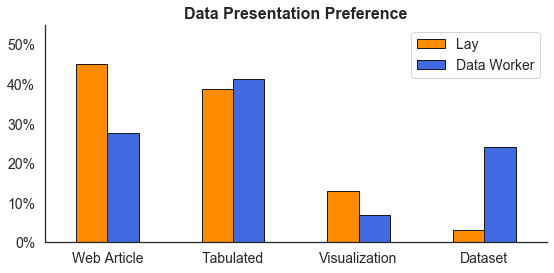
\includegraphics[width=0.9\columnwidth]{figures/datapresentation.png}
 \caption{Data presentation preference comparison between lay citizens and data workers}~\label{fig:datapresentation}
\end{figure}

The data presentation preference vary between lay citizens and data workers, but due to our study limitations, we did not perform a statistical comparison of the differences. However, Figure \ref{fig:datapresentation} suggests that lay citizens are very unlikely to look for information from raw datasets. The most common preference were articles which provide contextual information through words and numbers. There are some who are visual and would explore figures and charts.

\subsubsection{Data Interaction}
An additional behavior we noted from our observation of the participants was data interaction. In this study, we consider data interactions to be file downloads and data processing, such as filtering, aggregating, and sorting. Seven participants downloaded files in PDF and CSV formats but only three (N=3; DW1, DW3, L4) processed the raw data from ODPH.

Based on our observations, data workers leveraged on their experience to ensure the validity of their response through processing raw data, while the lay participants prefer already processed data presented in tabulated reports. We believe that this emphasizes the gap between the information seeking and sensemaking behaviors of experienced data workers and lay citizens.

% RQ3: How effective are Open Data Philippines and Freedom of Information portals in supporting the information seeking and sensemaking needs of the citizens?

% These behavioral observations can be classified into three categories: (1) No Scrolling in Freedom of Information; (2) Search via the Themes in Open Data Philippines; (3) Search via the Agency Open Data Philippines. The first checks whether or not the participant scrolled down the request page in order to look for the answer. The second counts the number of participants who navigated the Open Data Philippines website via the themed icons. Themed icons are topics that encompasses several datasets. For example, datasets that are fire related and typhoon related are found under the "Disaster and Rehabilitation" theme. The third counts the number of participants who navigated the website through the agency list feature found in Open Data Philippines. 

% To fully evaluate the efficacy of the Open Data Philippines and Freedom of Information portals (RQ3), we looked at the responses of the interviewees to identify the features that supported and restricted them from completing the tasks. These are found under our insightful observations classified under our In Vivo coding. These insightful observations can be categorized into three: (1) Feedback given on the use of both Freedom of Information and Open Data Philippines portals; (2) Feedback given on the use of Freedom of Information; and (3) Feedback given on the use of Open Data Philippines. For the first category, we further sub-categorize these kinds of feedback into five: (a) Lack of Granularity, where the participant expressed the lack of spatial and temporal components in the dataset they found; (b) Answer not Obvious, where the participant expressed that they cannot easily find the answer in the dataset they found; (c) Feedback and Recommendations, where the participant wanted some form of feedback even though their search query returns zero results; (d) Language Barrier, where the participants expressed that they want these websites to be in the native language as well; and (e) Addition of Visual Aids, where the participant expressed the need for infographics to easily understand the trends and behaviors found in the dataset. For the second category, we also further sub-categorize these feedback into four: (a) Keywords, where the participants felt like their use of keywords in the search engine are incorrect; (b) Compared to Google, where the participants compared the search engine of Open Data Philippines to Google's; (c) Unoptimized Search Engine, where the participants were unsatisfied with the search engine of Open Data Philippines; and (d) Likes Themes, where the participants express they liking towards the themed icons. For the third category, we also further sub-categorize these feedback into four: (a) Lack of Active URLs, where the participants felt like the website needed active URLs rather than just URLs in plain text; (b) No Themes, where the participants expressed their want of themed categories similar to Open Data Philippines; (c) Conversation Structure-B, where the participants expressed their dislike towards the conversation structure the website uses to display requests; and (d) Conversation Structure-G, where the participants expressed their liking towards the conversation structure the website uses to display requests. We then analyzed and looked at the way our interview respondents ranked the 6 different datasets to see how the look for information given a certain dataset and understand what kind of data they prefer to look at.

% Do we want to use feasibility or efficacy?
\subsubsection{Feasibility of Open Government Data Portals}
To determine whether OGD portals are feasible information seeking and sensemaking tools, we mainly use our results from the usability experiments on ODPH and eFOI. We found that these portals currently do not aid in the completion of the information seeking tasks provided, despite the availability of the information in those portals. We first look into the quantitative metrics of success in completing the tasks. We then expound on the insights from our interviews from two aspects: \textit{design and functionality} and \textit{data presentation and quality}.

As seen in the descriptive statistics in Table \ref{tab:participants}, data workers have a higher overall success rate for both portals as compared to the lay participants. We conducted a $\chi^2$ test of independence on their success and their awareness of the portal prior to the study and found that success is independent of the awareness. Looking at the time taken for those who were unsuccessful, participants gave up earlier on the ODPH tasks as compared to eFOI. 

%However, both groups have a relatively lower success rates in comparison to the web search.

% When considering the average time taken in performing the tasks, those accomplished using open government data platforms took more time compared to the interviewees' tool of choice. For Open Data Philippines, tasks that were not accomplished took less time than tasks not accomplished using their tool of choice. This indicates that these tasks may have not been accomplished due to majority of users giving up or believing that the platform did not have the information necessary to do the task. 
% Tasks that were not accomplished using FOI took the most amount of time, which could indicate the interviewees maximizing the allocated time limit or taking a longer amount of time before conceding. Overall, open data platforms may not be as effective in supporting the information seeking of the interviewees even though these platforms serve as repositories of data that can be accessed by any individual.

\subsubsection{Design and Functional Insights}
We primarily used the insights from our interview results to qualitatively evaluate the efficacy of the portals. Our results show that the \textit{unoptimized search engine} in both portals and the \textit{conversational design} of eFOI were common factors that hinder the participants in finding the datasets. However, \textit{categorical filters} of ODPH showed promise in supporting the search efforts of some participants. 

\textit{Unoptimized Search Engine}. Most of our respondents primarily used the search bar feature found in the website. Majority (N=16) of our participants expressed their frustrations with the unoptimized search engines of the portals mainly because the queries they used would return no results. DW2 was disappointed and assumed that the data was unavailable \textit{"because nothing really came up though the words were generic"}. L6 \textit{"was very hopeful"} but also got no results and gave up.

% L6 also expressed the same sentiment:
% \begin{quote}
% I was very hopeful but then nothing popped up. Stressful since nothing from the search terms popped up. 
% \end{quote}

Almost half (N=10) of our participants compared the search functionality of the portals to Google. When participant L4 was asked why he changed the structure of his search query in one of the tasks, he responded:
\begin{quote}
The second one [query] was just a change of order in the words since I don't know what logic is being used by Open Data. It could already be a set one unlike Google which is more powerful, more flexible.
\end{quote}

Three participants (N=3; L4, L6, L9) believed that their existing search behavior on Google would work on the open data portals as well:
\begin{quote}
Initially I did not understand how to use the open data Philippines. I thought it was like Google that you type in all your keywords. -- L9
\end{quote}

At least four (N=4; L6, L7, L8, L9) participants, who were also unaware of ODPH prior to the interview, noticed that it was very strict with the keywords since their queries had to exactly match the titles of the dataset. 
\begin{quote}
I found out it was easier to type in one keyword and [that] one specific keyword that would really encompass your whole search. -- L9
\end{quote}

\textit{Conversational Structure}. Upon viewing a request on eFOI, the conversation between the requester and the FOI officer is shown. If the request is approved, the data requested is usually found at the end of the page which requires users to scroll down the page. We observed the behavior of our participants during the eFOI tasks and only two participants (L4, SL1) did not scroll down the page.

% (DW3, L3, L4, L6, L11)
When probed about their experience on eFOI, five participants disliked the conversational structure. Two participants were unsure of what to do when presented with that interface. L6 specifically asked, \textit{"What am I gonna do with this?"}. 

% Both DW3 and L6 were unsure of what to do when they were presented with that interface.
%\begin{quote}
%Oh, at first when I searched in FOI, it was like conversation so I was like "What am I gonna do with this?" It's like you really have to read through it so you'd be able to, you know, get what you're searching for. -- L6
%\end{quote}

An additional concern three participants (L4, L11, DW7) noticed with the conversational structure was the lack of hyperlinks in the text. They could not easily see the link to the dataset provided in the conversation. Specifically, L4 mentioned that, \textit{"It took some getting used to, I was looking for hyperlinks actually."}

%\begin{quote}
%It took some getting used to, I was looking for hyperlinks actually. If I saw hyperlinks, especially if the interface of the hyperlink was a website address. -- L4
%\end{quote}

However, two participants (N=2; DW2, L11) liked this structure. They noted that it allowed the website to release credible and reliable data. When asked for the reason, DW2 said:
\begin{quote}
  Actually, it wasn't something that I was expecting from a Philippine website cause most of the times it's very impersonal (template response) but this one its kinda more personalized, I should say, and they're very polite.
\end{quote}

\textit{Categorical Filters}. ODPH has categorical icons below the search bar. When clicked, users will be provided a list of datasets under that category. Only seven participants used this feature while searching and three of them (N=3; L5, L7, DW5) expressed their interest in the categorical icons as an alternative way to search for data. In the previous design, the icons were not visible on load which suggest that this feature may be underutilized. Incidentally, L1 also used the categorical icons in ODPH and noted that he wanted a similar feature to be present in eFOI to provide users an alternate method of navigation.

% Only participants L5, L7, DW5 expressed their liking towards the theme icons found in the website as an alternative way to search for data. Specifically, participant L5 mentioned that "The categories were a nice tool."

% Have to rethink where to place this
% \subsubsection{Dataset Rankings}
% Since ODPH and eFOI have data in either dataset or processed tabulated form, we asked our participants to look into six unique datasets. They were then tasked to rank those datasets with the ranking criteria being totally dependent on them. We analyzed their responses for the purpose of understanding how they make sense of data. Majority of the participants ranked the data based on how useful they felt the data was to Filipino citizens. Consequently, the top 2 datasets that were ranked were traffic data from both roads and trains. This suggests that the participants find traffic data useful for Filipino citizens. Additionally, more lay people ranked the datasets based on how useful it would be for the common good and some lay people ranked the data based on the quality of it. In contrast, the data workers mostly ranked the datasets based on the structure of the dataset.

\subsubsection{Data Presentation and Quality Insights}
In addition to the portal features, we also requested our participants to describe the datasets found and their usefulness. Our results show that participants value \textit{straightforwardness}, \textit{granularity}, \textit{visualization}, and \textit{relevance} when it comes to data, regardless of data experience.

% \textit{Answer not Obvious}.
% L1, L5, L6, L7, L9, L10, DW3, DW6, DW7, DW8
\textit{Straightforwardness}. Almost half (N=10) of the participants felt that the answer to the task is not easily found in a dataset available in the OGD portals. Some form of processing is required to extract the needed information. DW7 specifically pointed out the challenge ordinary citizens face with raw datasets:
\begin{quote}
A layperson with no knowledge of statistical tools would not go further than the data presented to him. The websites won't spoon feed you with the data, you need to perform a little aggregation.
\end{quote}

In fact, two lay respondents (L7, L10) felt overwhelmed with the data found and were unsure of what to do with it. When asked what would make the task easier, L10 said: \textit{"I felt information overload. I want to see the data in a simpler way."} Additionally, L9 also thought that \textit{"brief and basic discussions of information"} would help.

In addition, at least four (N=4; L1, L4, L6, DW5) participants wanted data presented in an organized summary of information with clear labels. Both L1 and DW5 specifically mentioned the importance of \textit{"how easy it is to understand the data"}.

% "It's not common knowledge that you have to open the whole thing and stretch the dataset to see what it's trying to say" -L1

% “I don't like it to be honest, kase diba money kase ito, di sya nakaformat na maayos. Di mo maintindihan in first glance. Tapos ung iba na di mo magegets (PSGC).” -SG

\textit{Granularity}. Eight participants felt that the datasets they encountered were lacking and incomplete in terms of both spatial and temporal granularity. Three (N=3; L11, DW3, DW4) participants greatly valued granularity for both the post search evaluation and the dataset ranking. DW4 explained that \textit{"there is a lot more flexibility in your analysis"} when granular data is made available.

\textit{Visualization}. ODPH has a dataset preview which allows a user to explore the dataset in grid or graphical form. A participant (L5) wanted to view the data he found in a graph, however it took longer than expected to load so he attempted to graph it himself. Five other participants also suggested that infographics and other types of visualizations would be \textit{"helpful"} and \textit{"appealing"}. Detailed insights about visualizations came mostly from data workers who understand the value of visual representation of data. 
\begin{quote}
Visualizations, those are helpful because, for example, I'm looking for a trend in historical data, 50 years, 40 years ago. It's helpful to see that kind of trend" -- DW1 (translated from Tagalog to English)
\end{quote}

\textit{Relevance}. During the dataset ranking, nine of the participants placed importance on the relevance of the underlying information in the data to either their personal interests (DW6, DW7, SL1)  or perceived interests of fellow citizens. Specifically, L8 mentioned that, \textit{"This data can be useful for ordinary citizens especially traffic, police reports"}

%\begin{quote}
%  This data can be useful for ordinary citizens especially traffic, police reports. -- L8
%\end{quote}

% Have to rethink where to place this
% \subsubsection{Dataset Rankings}
% Since ODPH and eFOI have data in either dataset or processed tabulated form, we asked our participants to look into six unique datasets. They were then tasked to rank those datasets with the ranking criteria being totally dependent on them. We analyzed their responses for the purpose of understanding how they make sense of data. Majority of the participants ranked the data based on how useful they felt the data was to Filipino citizens. Consequently, the top 2 datasets that were ranked were traffic data from both roads and trains. This suggests that the participants find traffic data useful for Filipino citizens. Additionally, more lay people ranked the datasets based on how useful it would be for the common good and some lay people ranked the data based on the quality of it. In contrast, the data workers mostly ranked the datasets based on the structure of the dataset.

\section{Discussion}
We address our research questions by summarizing and corroborating the results from our climate survey and usability experiments. We then suggest policy recommendations to promote publication of OGD. Finally, we conclude by contributing design guidelines for how OGD portals can address barriers for citizen engagement. 

In summary, the results from our interviews corroborate the initial findings from the climate survey. Generally, citizens are interested in information that directly affect their daily lives, such as transportation and safety. Some participants believed that some of the available data in the open data portals are useful and relevant to themselves and others. Upon introduction of the portals to participants, some were surprised and initially thought it would be a useful source of information. However, based on the insights and our data inventory analysis, available open data can only address a limited range of interest of the general public (RQ1). Available data were mostly incomplete and outdated. 

In terms of the information seeking behavior of citizens, regardless of data experience, participants from both survey and interview still relied heavily on Google to find needed data or information as seen in previous studies \cite{Koesten2017}. However, slight differences were noted in the sensemaking behavior of data workers and lay citizens. Data workers would leverage on their knowledge of data processing to take that extra step to generate information while lay people preferred to have information readily available in articles or tabulated form.

The survey findings about the impracticality of current OGD portals, especially eFOI, are reinforced by the results of the interview tasks. Participants found it challenging to search for datasets in both ODPH and eFOI due to some ineffective design and functional implementation. Despite the existence of an exploratory visualization feature in open data portals, it was found to be underutilized and not user-friendly as it required prior background in data analysis. These findings show that there are improvements which could be made to these portals which could help in making it easier for people to find the data they need (RQ3). Improving the quality of these portals could result in more people using them when looking for data, which in turn could also help make people more aware of these portals \cite{corrales2019knowledge}.

% Furthermore, visual representation of raw data was a common request from participants which supports the findings from previous studies that visualizations are effective means of communicating data to a wider audience \cite{Erete2016}

% \subsection{Availability of Data in Open Government Data Portals}
% We found that Filipino citizens rank available datasets by their usability to other citizens and are more interested in categories of data that affect their personal lives. Moreover, findings from the data inventory state that majority of the interests of citizens are not available on open government data portals. These findings show that Filipino citizens have a small chance of finding data that interests them within ODPH and eFOI. Therefore, the availability of these open government data portals are lacking in data that interest Filipino citizens and we suggest increasing the amount of data that affect citizens to increase use of open government data portals \cite{Puussaar2018}.

% \subsection{Awareness of Open Government Data Portals}
% Results from both the interview and the survey show that data workers are more familiar with ODPH and eFOI compared to our non-data worker respondents. However, among all respondents, more respondents are aware of ODPH than eFOI. These findings show that outside the group of those who regularly perform data analysis, the existence of open government data portals is largely unknown. Therefore, we recommend that work should be done to increase lay people's awareness with these Open Government Data portals. 

% \subsection{Efficacy of Open Government Data Portals}

\subsection{Policy Recommendations for Citizen Engagement}
Open government data provides an avenue to promote citizen engagement. Civic hackers use open data to develop software and tools with the aim of providing better understanding of available data \cite{Choi2017, Puussaar2018, Robinson2016}. We provide empirical results that suggest that an \textit{abundant} OGD portal could promote citizen engagement provided that certain \textit{design and functional improvements} are implemented. To support the information needs of citizens, we propose that policies be implemented (1) to increase the publication of high quality reliable data in open license formats and (2) to promote awareness among citizens. 

\subsubsection{Increase Publication}
Based on the insights from the interviews, we found that data workers are interested in analyzing government data for social good as long as that the data provided have higher spatial and temporal granularity. Participants also believed that some data are already relevant to their personal lives and their community. To further support the information needs of citizens, we propose the implementing agency to provide data creation and publication guidelines for different branches of government to follow. In addition, quality control processes should be included in the publication pipeline to ensure compliance to the guidelines and other ethical concerns, such as data privacy. Some eFOI data requests are provided with PDF files, however, this format is not considered open standard since it is not machine-readable. The national government could potentially incentivize agencies that respond to eFOI requests with machine-readable data or information. 

\subsubsection{Promote Awareness}
Majority of the participants from both studies were unaware of the open data initiatives of the Philippines. However, once introduced to the portals, some participants were enthusiastic and expressed interest in the data they encountered. Exposure to the portal generated insightful feedback from both data workers and lay citizens which suggests that an increase in awareness among citizens might enable citizen engagement. Civic hackathons could be organized to utilize available open data and to provide feedback on further data improvements for the government \cite{Robinson2016}. A number of our interviewed participants (N=5) suggested these portals be advertised in social media and news outlets. Future longitudinal research may be done to evaluate the effects of increased awareness on citizen engagement.

\subsection{Design Implications to Support Information Seeking and Sensemaking}
% Metadata, UX, and other choo-choo. Maybe separate it based on foi and odph?
In the context of HDI, it is important that the presentation of data be legible for concerned parties to allow ease of understanding of the data provided to them \cite{Mortier2014}. Since ODPH and eFOI should cater to all Filipino citizens, it is important that these sites provide data in a legible manner. Our results show that citizens would benefit from (1) improved search options and (2) visualized, contextualized, and processed content for better sensemaking. We also present localized design enhancements which cater to the Philippine OGD portals specifically.

\subsubsection{Improved Search Options}
Both our results and previous literature \cite{kacprzak2019characterising} suggest that existing search techniques from web search does not apply to dataset search. Although some of the participants were able to adapt to the built-in search engine, we recommend that the search engine be optimized to enable faster and more efficient searches. Alternatively, better placement of existing filtering features may also improve the search process of users. In addition, as spatial and temporal keywords were common in search queries, we also recommend that the search engine look through the metadata of uploaded datasets. This would also require proper documentation of published datasets which may only be controlled by the data provider.

\subsubsection{Visualized and Contextualized Content}
Our results show that citizens, regardless of data experience, prefer a straightforward answer when seeking information. To support this, we emphasize the need for descriptive visualizations to communicate the content of the dataset to both types of users. The majority of our lay participants wanted visual aids to help them understand what the values in the datasets mean. OGD publishers could provide preliminary charts or summarized tables that present information instead of raw data. Although storytelling and visualizations have been determined effective in communicating data \cite{Erete2016}, further research is needed to understand how Filipinos perceive data visualizations as previous literature suggests that various factors affect the attitude and perception of individuals about visualizations \cite{Peck2019}. 

\subsubsection{Localized Design Enhancements}
Participants were not particularly embracing of the conversational feature of eFOI since it did not highlight the data's existence. We recommend a redesign of the portal to focus on the \textit{availability} of the data requested instead of the \textit{status} of the request. 

The Philippines has two official languages, English and Filipino. However, not all citizens are proficient in English. Two of our participants expressed the need for these official government portals to have \textit{bilingual capabilities}. Although it seems like this design suggestion is specific to the Philippines, we believe that this may also be applicable to other countries that have official multilingualism polices in place.
% Second, the Open Data Philippines website needs further improvement on their search engine since their search engine was highlighted to be strict with the kinds of results it would return. In the case that it would take much time and effort to optimize the said search engine, we recommend the website to put emphasis on other navigation features of the website such as the categorical filters and agency search wherein the user may look at datasets under certain categories and under certain agencies respectively. Participants who used these features during the usability experiments were reported to have higher success rates in finding the data they needed. Finally, we recommend that the Freedom of Information website to not present its data in a conversation-like structure since the majority of our participants were unsure of what to do upon seeing the said structure. It was not first instinct to find the data in the conversation between the requester and respondent. We further recommend Freedom of Information to put emphasis on the data provided rather than the conversation between the requester and respondent.


% \subsection{Information Seeking Behaviour}
% Based on the findings from the usability tests, there exist opportunities for open data portals to better cater to users' information seeking behavior. As searching for datasets using a combination of spatial and temporal keywords was seen to be the prominent method of information seeking by lay citizens, we recommend the optimization of open data portal search engines that would search through the metadata of datasets to return the most relevant results. Users were also found to be discouraged when finding no relevant data returned to them as a result of their search. We recommend a system that can provide related or similar datasets as a search result in the case that the exact data being searched for does not exist. Finally, it was also evident that lay citizens have a preference for tabulated and textual presentation of data over raw datasets. We recommend open data portals to provide visualizations and data stories to provide lay citizens with meaningful insights without requiring background in data analysis.


\begin{comment}
% Maybe these design suggestions can be added in the design guidelines instead
\textit{Other Overall insights}. Three participants (N=3; L8, DW1, DW2) felt the need to have some form of feedback or recommendation when their search query returned no results in Open Data Philippines and in Freedom of Information. Participants would comment on how hopeful they were with what kinds of data these portals had but were disappointed with what their search queries returned them. Participant mentions that, "For example in Open Data [website], it would have been easier if there were recommendations, not entirely giving the person searching for answers a zero result. Cause if that happens, it's kind of discouraging to use the website." Participant DW1 even made a recommendation for the Open Data Philippines website by saying, "For example, when I'm in Open Data PH, when you start typing, if I'm on the second or third letter, there should be a recommendation, so I think that's helpful [Translated from Tagalog to English]." Only two participants (N=2; L8, L11) felt the need to have the Open Data Philippines and Freedom of Information websites in the Philippine native language as these websites were in English. Additionally, they mention that these websites should also be available in the vernacular language so that these open data websites can be used by the general public. Participant L8 mentions that, "For starters, it [the open data websites] should be in Tagalog so that it is easily understandable so that it will be easier to understand it and it can be bilingual anyways [Translated from Tagalog to English]."
\end{comment}

\section{Limitations}
We acknowledge that a longer-term study that examines the information needs and behavior of more participants could provide a more comprehensive understanding of the information seeking and sensemaking behavior of lay citizens. This would also allow for further comparison between different samples of the population. We also acknowledge that a more statistical approach of sampling for the survey could give us a better representation of the population's information needs. Although the portals tested were only Open Data Philippines and the Freedom of Information request portal, our analysis of the information seeking behavior of lay citizens strengthens our confidence that open government portals should consider a more lay citizen friendly design to support citizen engagement.

\section{Conclusion and Future Work}
We conducted a climate survey of 119 respondents to understand their information needs and their awareness of the open government data portals provided by the Philippine government. We also sought to quantify whether these information needs are answerable by available open government data by cross validating the results of the survey to the data in Open Data Philippines and Freedom of Information portals. We also investigated the information seeking behavior of 13 lay citizens and eight data workers to compare the behavior of both groups. In addition, we also conducted usability tests and semi-structured interviews with these 21 participants to identify gaps in the design of the two portals. We found that only some information needs of lay citizens are answerable by currently available open government data. However, these datasets only provide partial answers to the specific questions relevant to the citizens. We also found that lay citizens would benefit from localized and advanced search engines, visualized, contextualized, and processed content for better sensemaking. We contribute design opportunities to promote lay citizens in understanding of available open government data. Our findings and implications emphasize the importance of a citizen-driven design of open government data portals to increase citizen engagement in open government initiatives.

Moving forward, we would like to design and test prototypes to understand whether our design guidelines promote better understanding of available open government data. If this proves successful, we would like to conduct a longitudinal study to examine if this leads to an increase in citizen engagement with the government. 

\begin{comment}
\section{Acknowledgments}
Sample text: We thank all the volunteers, and all publications support
and staff, who wrote and provided helpful comments on previous
versions of this document. Authors 1, 2, and 3 gratefully acknowledge
the grant from NSF (\#1234--2012--ABC). \textit{This whole paragraph is
 just an example.}
\end{comment}


% Balancing columns in a ref list is a bit of a pain because you
% either use a hack like flushend or balance, or manually insert
% a column break. http://www.tex.ac.uk/cgi-bin/texfaq2html?label=balance
% multicols doesn't work because we're already in two-column mode,
% and flushend isn't awesome, so I choose balance. See this
% for more info: http://cs.brown.edu/system/software/latex/doc/balance.pdf
%
% Note that in a perfect world balance wants to be in the first
% column of the last page.
%
% If balance doesn't work for you, you can remove that and
% hard-code a column break into the bbl file right before you
% submit:
%
% http://stackoverflow.com/questions/2149854/how-to-manually-equalize-columns-
% in-an-ieee-paper-if-using-bibtex
%
% Or, just remove \balance and give up on balancing the last page.
%
\balance{}
% BALANCE COLUMNS
\balance{}

% REFERENCES FORMAT
% References must be the same font size as other body text.
\bibliographystyle{SIGCHI-Reference-Format}
\bibliography{sample}

\end{document}

%%% Local Variables:
%%% mode: latex
%%% TeX-master: t
%%% End:
